\section{Introduction}
% ==============================================
Code reuse via copying and pasting is a common practice in software development~\cite{Kim2004, Jiang2007, Li2004}. Prior studies show that up to 25\% of code in modern software contains {\em code clones}\textemdash code similar to other code fragments elsewhere~\cite{baker1995finding, Al-Ekram2005:byaccident, roy2008empirical}. Manually adapting clones is error-prone. Chou et al.~show that a large portion of operating system bugs is introduced by manual porting mistakes between clones~\cite{Chou2001}. Juegens et al.~find that ``nearly every second unintentionally inconsistent change to a clone leads to a fault''~\cite{juergens2009code}. Therefore, developers may want to examine and contrast runtime behavior of clones. Fischer finds that developers want to see how reused code works in terms of runtime behavior~\cite{fischer1987cognitive}. Holmes et al.~find that developers want to leverage existing tests to validate reused code~\cite{holmes2007supporting}. We also find that industrial developers rely on regression testing to check for inconsistent or missing edits on clones~\cite{zhang2015interactive}.

However, the situation is exacerbated due to a lack of tests, where some clones are tested while their counterparts are not. In fact, our study shows that, in 46\% of studied clone pairs, only one clone is tested by existing tests, but not its counterpart. No existing techniques can help programmers reason about runtime behavior differences of clones, especially when clones are not identical and when clones are not tested. In the absence of test cases, developers can only resort to static analysis techniques to examine clones~\cite{Li2004, Jiang2007, Pham2010:vulnerability, Ray2013:spa, zhang2015interactive}, but these techniques are limited to finding only pre-defined types of cloning bugs such as renaming mistakes or control-flow and data-flow inconsistencies.

%This paper presents a test reuse and differential testing framework for clones, called {\grafter}. Given a pair of clones and an existing test suite, {\grafter} helps programmers cross-check runtime behavior via code grafting and differential testing. To reuse tests for similar but not identical code, {\grafter} grafts one clone in place of another to exercise the grafted clone using the same test as the original clone. We make this choice of transplanting clones instead of tests, because we target clones appearing in the middle of a method without a well-defined interface (i.e., explicit input arguments and return type), which are often found by widely-used clone detectors such as Deckard~\cite{Jiang2007} or CCFinder~\cite{Kamiya2002}. {\grafter} exposes the de-facto interface of a clone by identifying input and output objects, grafts the clone, and propagates intermediate input data to establish the same test environment.

This paper presents a test reuse and differential testing framework for clones, called {\grafter}. Given a pair of clones and an existing test suite, {\grafter} helps programmers cross-check runtime behavior by exercising the clones using the same test. Test reuse for clones is challenging because clones may appear in the middle of a method without a well-defined interface (i.e., explicit input arguments and return type), which also makes it hard to directly adapt test for reuse. Such intra-method clones are often found by widely-used clone detectors such as Deckard~\cite{Jiang2007} or CCFinder~\cite{Kamiya2002}. {\grafter} identifies input and output parameters of a clone to expose its de-facto interface and then grafts one clone in place of its counterpart to exercise the grafted clone using the same test.

\begin{figure}[!t]
\centering
\includegraphics[width=0.5\textwidth]{overview.pdf}
\caption{The overview of Grafter}
\label{fig:output}
\vspace{-4mm}
\end{figure}

%\begin{figure*}[!ht]
\begin{minipage}[t]{0.49\linewidth}
\begin{lstlisting}[style=MyJavaSmallStyle]
public class Copy extends Task{
 private IncludePatternSet includes;

 public void setIncludes(String patterns){
   ...
   if(patterns != null && patterns.length() > 0){
-    StringTokenizer tok=new StringTokenizer(patterns,",");
-    while(tok.hasMoreTokens()){
-      includes.addPattern(tok.next());
-    }
+    String[] tokens = StringUtils.split(patterns, ",");
+    for(String tok : tokens){
+      includes.addPattern(tok);
+    }
   }
 }
  ...
}

public class IncludePatternSet{
 public Set<String> set;
 public void addPattern(String s) { set.add(s); }
  ...
}

\end{lstlisting}
\vspace{-2mm}
\begin{center}\begin{footnotesize}(a) Correctly edited clone in the Copy class\end{footnotesize}\end{center}
\end{minipage}
%
\begin{minipage}[t]{0.49\linewidth}
\begin{lstlisting}[style=MyJavaSmallStyle]
public class Delete extends Task{
 private ExcludePatternSet excludes;

 public void setExcludes(String patterns){
   ...
   if(patterns != null && patterns.length() > 0){
-    StringTokenizer tok=new StringTokenizer(patterns,",");
-    while(tok.hasMoreTokens()){
-      excludes.addPattern(tok.next());
-    }
+    String[] tokens = StringUtils.split(patterns, ".");
+    for(String tok : tokens){
+      excludes.addPattern(tok);
+    }
   }
 }
  ...
}

public class ExcludePatternSet{
 public Set<String> set;
 public void addPattern(String s) { set.add(s); }
  ...
}
\end{lstlisting}
\vspace{-2mm}
\begin{center}\begin{footnotesize}(b) Inconsistenly edited clone in the Delete class\end{footnotesize}\end{center}
\end{minipage}
\caption{Similar edits to update the use of {\ttt StringTokenizer} API to {\ttt StringUtils.split} in {\ttt Copy} and {\ttt Delete}.}% The programmer mistakenly changes the string separator from a comma to a period (line 11 in the {\ttt Delete} class). Code deletions are marked with `-' and additions are marked with `+'. }
\label{fig:example}
\vspace{-4mm}
\end{figure*}

\begin{figure}[!th]
 \centering
 \begin{lstlisting}[style=MyJavaSmallStyle]
@Test
public void testCopy(){
  Task copyTask = FileUtils.createTask(FileUtils.COPY);
  ...
  copyTask.setIncludes("src/*.java, test/*.java");
  JobHandler.fireEvent(copyTask);
  assertTrue(checkFileCopied());
}
\end{lstlisting}
\vspace{-3mm}
\caption{A test case for the {\ttt Copy} class.}% It copies java files in the src folder and the test folder to a target directory and checks if all matched files are copied by calling the {\ttt checkFileCopied} method.}
\label{fig:test}
\vspace{-6mm}
\end{figure}


\begin{figure*}[!th]
\centering
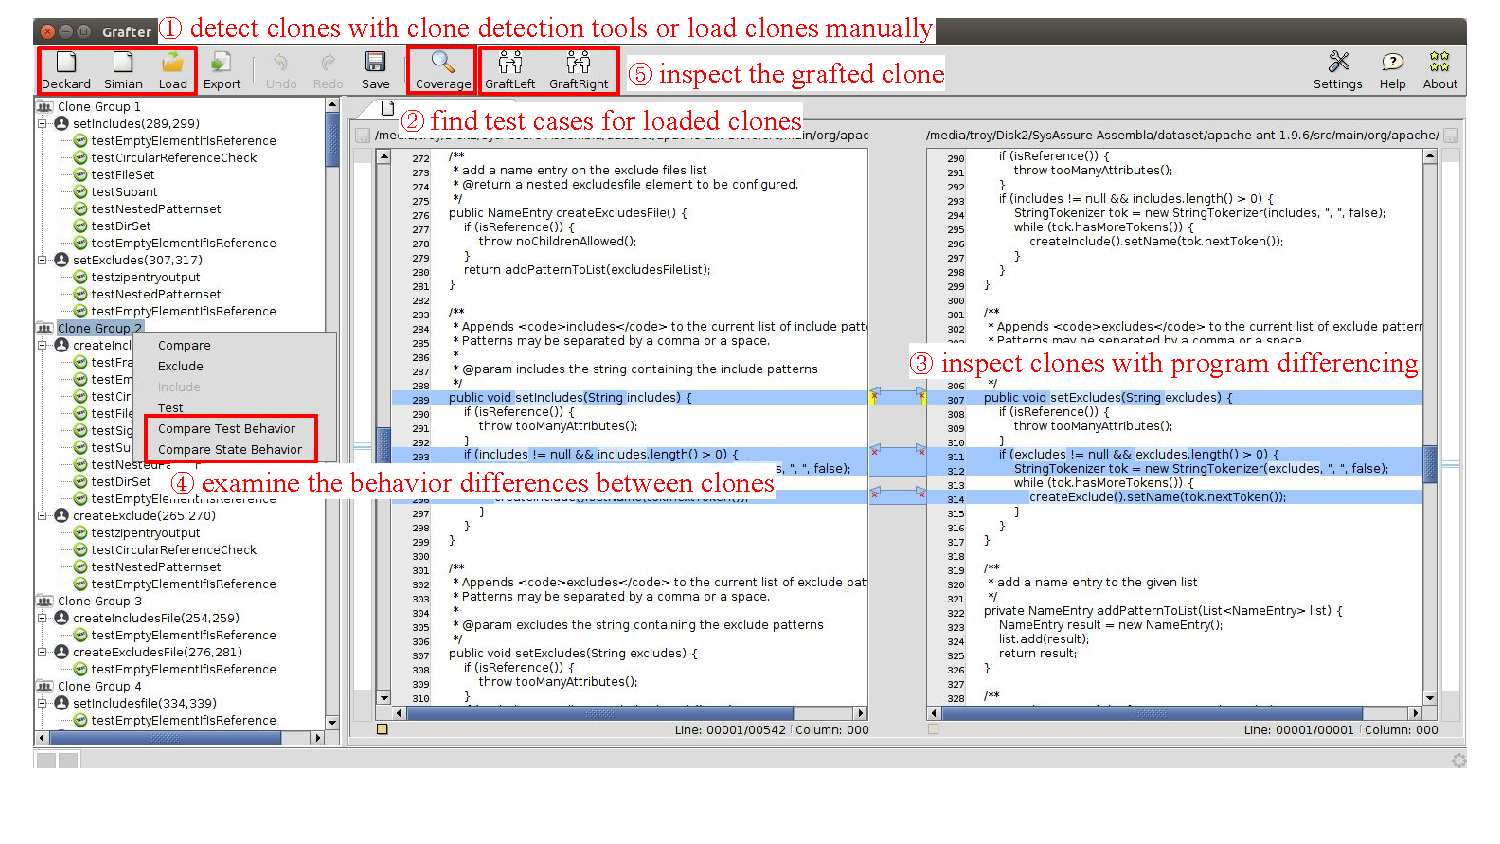
\includegraphics[width=\linewidth]{grafter-screenshot-v3.pdf}
\caption{The screenshot of Grafter}
\label{fig:screenshot}
\end{figure*}

Similar to how organ transplantation may bring incompatibility issues between a donor and its recipient, a grafted clone may not fit the context of the target program due to variations in clone content. For example, if a clone uses variables or calls methods that are not defined in the context of its counterpart, simply copying a clone in place of another will lead to compilation errors. To ensure {\em type safety} during grafting, {\grafter} performs inter-procedural analysis to identify variations in referenced variables and methods. It then adapts the grafted clone using five transplantation rules to handle the variations in referenced variables, types, and method calls. Finally, it synthesizes stub code to propagate input data to the grafted clone and then transfers intermediate outputs back to the recipient. {\grafter} supports differential testing at two levels: test outcomes (i.e., {\it test-level comparison}) and intermediate program states (i.e., {\it state-level comparison}). During differential testing, {\grafter} does not assume that all clones should behave similarly nor considers that all behavioral differences indicate bugs. In fact, a prior study on clone genealogies~\cite{Kim05} indicates that many syntactically similar clones are used in different contexts and have intended behavioral differences. The purpose of differential testing in {\grafter} is rather to illuminate and expose behavioral differences at a fine-grained level {\em automatically} and {\em concretely} by pinpointing which variables' states differ in which test.
 
We evaluate {\grafter} on 52 pairs of nonidentical clones from three open-source projects: Apache Ant, Java-APNS, and Apache XML Security. % To assess {\grafter}'s ability to reuse tests for nonidentical clones, our dataset includes 38 pairs of syntactically identical code fragments except for variations in variables, types, and methods, etc, and 14 pairs are similar code fragments with further variations such as added or deleted statements. 
 {\grafter} successfully grafts and reuses tests in 49 out of 52 pairs of clones without inducing compilation errors. Successfully reusing tests in 94\% of the cases is significant, because currently no techniques enable test reuse for nonidentical clones appearing in the middle of a method. {\grafter} inserts up to 33 lines of stub code (6 on average) to ensure type safety during grafting, indicating that code transplantation and data propagation in {\grafter} are not trivial. To assess its fault detection capability, we systematically seed 361 mutants as artificial faults using the {\major} mutation framework~\cite{just2014major}. We use Jiang et al.'s static cloning bug finder~\cite{Jiang2007} as a baseline for comparison. 
By noticing runtime behavioral discrepancies, {\grafter} is more robust at detecting injected mutants than Jiang et al.\textemdash 31\% more using the test-level comparison and almost 2X more using the state-level comparison. {\grafter}'s state-level comparison also narrows down the number of variables to inspect to three variables on average. Therefore, {\grafter} should complement static cloning bug finders by enabling runtime behavior comparison. Our grafting technology may also have potential to assist code reuse and repair~\cite{weimer2009automatically, Barr2015AST, petke2014using, harman2014babel}. 